%======================================================================
\chapter{Introduction} \label{chapters:intro}
%======================================================================

In 1977 Sanger {\em et al.} \cite{sanger} published their results describing the usage of dideoxynucleotide termination DNA sequencing technology and, thus, formed formed the basis for DNA sequencing. Since this initial development there have been countless improvements in sequencing technology by drawing on advancements in molecular biology, chemistry, and computer science.  With the development of high-throughput next generation sequencing technologies has arisen large amounts of genomic data, and an increased need for novel ways to analyze this data. The growing amount of data makes it impossible to analyze DNA sequences manually. 

This revolution in DNA sequencing technologies has led to many new challenging problems in bioinformatics. For example, the human genome contains over three billion building blocks called nucleotides, which are represented by the symbols A, C, G, and T.  Due to the immense size of this dataset, it is infeasible to analyze this data manually and biologists must use computational methods to find novel, functional regions. In order to begin to answer some of these problems in bioinformatics, we need to abstractly and realistically model these problems as discrete objects.  This thesis will focus on one such model, the development of efficient algorithms for that model, and the application of these algorithms to analysis of genomic data. 

Short substrings of genomic data that are responsible for biological processes, such as gene expression, are referred to as {\em motifs}.  Motifs with the same function may not entirely match, due to mutation events at a few of the motif positions. Given a number of DNA strings, the motif-recognition problem is the task of discovering motif instances in every given string without knowledge of the position of the instances or the pattern shared by these substrings.  Motif recognition is a NP-complete problem, and therefore it is unlikely that there exists a polynomial-time algorithm for this problem. Since finding motif instances using laboratory methods is an extremely costly and lengthy process, it is vital to create accurate and efficient computational methods to assist in finding possible motif instances. The aim is to develop an application that will find possible motif instances; the user then must decide whether these instances warrant further biological investigation based on their statistical significance. Numerous algorithms and programs have been developed to find motifs in DNA sequences but many have limited accuracy or computational tractability \cite{BT02,PS00}.

In Chapter \ref{chapter:mclwmr}, we describe a novel approach to motif recognition, and provide theoretical and experimental results that demonstrate its efficiency and accuracy. Our algorithm, MCL-WMR, builds a weighted graph model of the given motif-recognition problem and uses a graph clustering algorithm to quickly determine important subgraphs that need to be searched further for valid motifs \cite{boucher07}. Previous algorithms and programs search exhaustively or probabilistically on an unweighted graph or sequence model of the input data, but due to the lack of information contained in these models, the required search is extremely broad and requires considerable computation time.  By considering a weighted graph model, we narrow the search dramatically to smaller problems that can be solved with significantly less computation.  An empirical comparison to previous work illustrates that MCL-WMR is a leading method with respect to its running time and accuracy.   This chapter is based on joint work with Daniel G. Brown and Paul Church \cite{boucher07}.

The {\sc Closest String} problem is a NP-complete problem related to the motif-recognition problem. In Chapter \ref{chapter:closest_string_problem} we study combinatorial and probabilistic algorithms for this problem, and consider two subgroups of the problem instances: where the number of strings is small, and where the number of strings is relatively large. We give a linear-time algorithm for the restricted version of {\sc Closest String} where the number of strings is small, a result which resolves an open problem described by Gramm {\em et al.}\ \cite{GNR03}. Next, we present a polynomial-time heuristic for the {\sc Closest String} problem, and give an analysis that proves the algorithm is extremely efficient when the number of strings is relatively large.  The key to obtaining this latter result is the application of smoothed analysis, an intermediate measure between average case analysis and worst case analysis; whereas average-case analysis studies the average behaviour of an algorithm over all instances of a problem, smoothed analysis studies the average behaviour of the algorithm on each ``local region'' of the instance space \cite{ST01}.  Section \ref{sec:small_CS_insances} of Chapter \ref{chapter:closest_string_problem} is based on joint work with Stephane Durocher and Daniel G. Brown \cite{boucher08}.  Section \ref{sec:large_CS_insances_v1} is based on part of the joint work with Kathleen Wilkie \cite{boucher2010_1}. 

In Chapter \ref{chapter:closest_string_problem} we also consider the $O(n\ell + nd \cdot d^d)$-time algorithm by Gramm {\em et al.}\ \cite{GNR03}, an algorithm that has been shown to work very efficiently in practice. We explain this good performance through smoothed analysis.  Imperative to our analysis is the introduction of a perturbation model of the {\sc Closest String} model and the probabilistic analysis of the $O(n\ell + nd \cdot d^d)$-time algorithm by Gramm {\em et al.}\ \cite{GNR03}. We show for any given {\sc Closest String} instance, the average running time of this algorithm on a small perturbation of the instance is $O(n\ell + nd \cdot d^{2 - \epsilon})$. 

In Chapter \ref{chapter:cswo} we investigate a slight augmentation of the {\sc Closest String} problem that is a more realistic model of several biological problems.  We give a systematic parameterized complexity analysis of this new model by considering several parameterizations of this problem.   We give a negative complexity result by showing that the problem is W[1]-hard for unbounded alphabet size and every combination of a subset of the problem parameters.  We also show that  when the alphabet is unbounded, there exists a fixed parameter tractable algorithm with respect to two of the problem parameters. This chapter is based on joint work with Bin Ma \cite{boucher_ma}. 

In Chapter \ref{chapter:pmclwmr} we describe the application and implementation of the combinatorial and probabilistic insights described in the previous chapter to motif recognition.  Applying these methods -- as well as other insights -- we develop sMCL-WMR, a program that is capable of detecting weak motifs in large datasets and is much faster than its predecessor MCL-WMR. Further, we show the capability of this program in detecting transcription factor binding sites in real biological data.  In addition, we include work concerning canola genomics that was completed in collaboration with researchers at the University of Alberta and the Alberta Research Council.  Canola exhibits several desirable nutritional and economic factors and therefore, is an important target for genomic research in Canada.  By developing and employing genomic tools, which include sMCL-WMR and MCL-WMR, we are capable of identifying important regions of the canola genome that are responsible for specific biological activities.  This knowledge may be used in the long-term aim of developing crop varieties with specific biological characteristics, such as being disease-resistant.  The importance of these results is two-fold; it illustrates the capability of MCL-WMR and sMCL-WMR, and contributes to the study of crop genomics.  This chapter is partly based on joint work with James King \cite{boucher_king}, and joint work with Limin Wu and Saleh Shah.

Finally, in Chapter \ref{chapter:conclusions} we conclude this thesis by outlining some related areas for future research.  The areas extend from extensive and well-researched fields (such as the {\sc Closest String} problem, and combinatorial methods for counting and sampling) to more interdisciplinary fields that require a careful search through diverse literature (such as finding biological applications to a variant of the {\sc Closest String} problem).  
  
In this rest of this chapter, we define the motif-recognition problem and several distinguishing string selection problems more formally, and motivate our study by giving several biological applications of these problems; one of these applications will be thoroughly explored in this chapter and Chapter \ref{chapter:pmclwmr}. 

\section{From Transcription Factors to Pattern  Recognition}

From a high level, motif recognition can simply be described as classifying patterns ({\em a.k.a.}\ motifs) based on a priori knowledge or statistical information extracted from the data.   Motif recognition is an important problem in biology; it and its variants have several important applications in bioinformatics.  Before describing motif recognition from a computational perspective, we give an example motivating the investigation of this problem.   

A {\em gene} is a region of DNA that codes for a type of protein or a RNA chain that has a function in the organism.  Regulation genes, first discovered in 1961 by Jacob and Monod \cite{monod}, are a type of gene that provides the instructions for creating proteins which help control the expression of other structural genes. Hence, we can think of a sequence of DNA coding for a particular protein that, due to the chemical properties of the amino acids it is made from, folds in a particular manner and so performs a particular function ({\em i.e.} enzymes, structural, regulatory). The protein encoding genes are regulated in the following three levels:
\begin{description}
\item[Transcription control level:] determines if the transcription can begin.
\item[Post-transcription control level:] occurs after the DNA is transcribed and mRNA.  Regulates how much the mRNA is translated into proteins by capping, splicing, and poly-adenylation. These processes occur in eukaryotes but not in prokaryotes. This modulation is a result of a protein or transcript which in turn is regulated and may have an affinity for certain sequences.
\item[Post-translation control level:] control on the protein level.  
\end{description}
 
We adopt the convention that a DNA molecule is represented as a sequence whose symbols come from the four different nucleotides A, C, G, and T, and a protein is represented as a sequence whose symbols come from the 20 different amino acids. 
  
All the above controls occur during distinct stages described in the {\em central dogma of molecular biology}, the axiom that genetic information flows from DNA to RNA to protein and and cannot flow in the reverse direction \cite{crick}.  Figure \ref{fig:central_dogma} illustrates this process. The conversion from DNA to RNA is known as {\em transcription}, whereas, the decoding of a messenger RNA (mRNA) sequence into an amino acid sequence is referred to as {\em translation}.  We will focus on transcription control.  

\begin{figure}[h!]
\begin{center}
 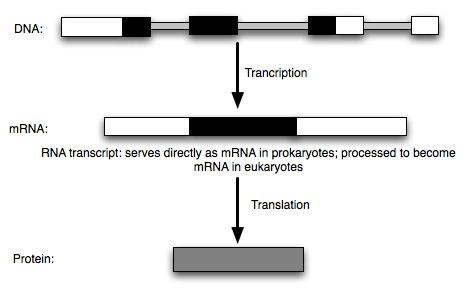
\includegraphics[width=\linewidth]{images/central_dogma}
\caption{An illustration of the flow of genetic information from DNA to RNA to protein. }
\label{fig:central_dogma}
\end{center}
\end{figure}

A typical genome contains protein coding genes, non-coding RNAs, regulatory sequences, which we refer to as {\em promoters}, and regions that have no known function or are yet to be classified. In this section, we will restrict interest to the promoter regions, which are DNA sequences near the beginning of genes that signal RNA polymerase where to begin transcription.  

The transcription process for a particular gene often requires that one or more transcription factors be bound to several specific regions, referred to as {\em binding sites}, that are located in the regulatory region of the gene.  A single transcription factor can be bound to multiple binding sites; however they must have similar length and nucleotide pattern.  This specific nucleotide sequence will compromise the regions of interest and will encompass a motif in the context of motif recognition. Typically, a binding site is between five to twelve nucleotides (nt) in length but could be as large as 30 nt \cite{BB05}.  Note that nucleotide sequences are virtually synonymous with a sequence of base pairs (bp). Figure \ref{fig:binding_site} illustrates a binding site with a bound transcription factor. 

\begin{figure}[h]
\begin{center}
 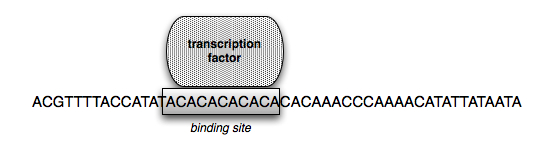
\includegraphics[width=\linewidth]{images/binding_site}
\caption{Depiction of a transcription factor binding site with bound transcription factor.}
\label{fig:binding_site}
\end{center}
\end{figure}

The discovery of motifs allows biologists to understand the complex mechanisms that regulate gene expression. A single transcription factor is often not sufficient for the regulation of transcription, and typically, there exists a set of transcription factors for a single gene.  The binding sites usually occur as a recurring pattern in the sequence of nucleotides, however, due to the possibility of genetic mutation, a specific binding site in a nucleotide sequence will sometimes mismatch with the identified nucleotide pattern at a number of positions.  Therefore, subsequences of a set of nucleotide data corresponding to the same binding site will likely not all match exactly, making the identification of these subsequences by computational means considerably more difficult.  

The process of determining transcription factor binding sites can be described by the following steps: 
\begin{enumerate}
\item Determine a set of promoters that contain the same binding site. This will be the input for the next step.  
\item Identify reoccurring subsequences in the data that are likely are to be of biological interest using computational methods.  
\item Experimentally evaluate the biological function of the subsequences identified in the previous step. Biological experiments to verify regulatory sites are tedious and time-consuming.  One approach is to mutate different combinations of nucleotides until the functionality of the sequence changes.  
\end{enumerate} 

We will briefly describe one method for the first of the steps in this process that uses co-expressed genes (genes that are expressed together). They are likely regulated by the same transcription factors and can be identified through clustering of microarray data. A microarray works by exploiting the ability of a given mRNA molecule to bind specifically to, or hybridize to, the DNA template from which it originated. An array containing many DNA samples can be used to determine (in a single experiment) the expression levels of hundreds or thousands of genes within a cell by measuring the amount of mRNA bound to each site on the array. With the aid of computational experiments, the amount of mRNA bound to the spots on the microarray is precisely measured, generating a profile of gene expression in the cell. Hence, using the microarray data we can find genes that are expected to be regulated by the same transcription factor, by measuring the level of transcription of mRNA based on presence or absence binding factors.

The second step listed above will be the main focus of this thesis.  Identifying transcription factor binding sites is one specific example that will motivate our study of motif recognition. We will return to this specific biological problem later in this chapter, and in Chapter \ref{chapter:pmclwmr}, but next we will more thoroughly describe motif recognition from a computational perspective.

%\section{Notation}

%Let $s$ be a string over the alphabet $\Sigma$.  $|s|$ denotes the length of $s$ and $s(j)$ denotes the $j$th letter of $s$.  Hence, $s = s(1)s(2)\ldots s(|s|)$. Given a set $S$ of $n$, $\ell$-length strings, the aim of the optimization version of the {\sc Closest String} problem is to determine a string $s$ that minimizes the maximum distance to any string in $S$.  Given a set of strings $S = \{s_1, \ldots, s_n\}$, each string of length  $\ell$, then a string $s$ is a {\em closest string} for $S$ if and only if there is no string $s'$ such that $\max_{i = 1, \ldots, n} d(s', s_i) < \max_{i = 1, \ldots, n} d(s, s_i)$.  If $S$ is a set of strings and $s$ is a closest string, we refer to the {\em optimal closest distance} $d$ as the Hamming distance $\max_{i = 1, \ldots, n} d(s, s_i)$.  We refer to a {\em majority vote} for $S$ as the $\ell$-length string containing the letter that occurs most often at each positions; note, that this string is not necessarily unique.  Lastly, we denote a function $g$ to be an asymptotic estimation of $f$ as $f \asymp g$.  

\section{The Motif-Recognition Problem}
 
The bioinformatics literature uses disparate terminology and notation to define and describe the problem of identifying binding sites in regulatory regions.  To facilitate our discussion, we begin with general definitions, then make these statements more formal when deemed necessary. 

Given a number of biological sequences, motif recognition is the task of discovering meaningful patterns from the data without any prior knowledge.  Consider a set of sequences $S = \{S_1, \ldots, S_n\}$.  The aim is to use a computational algorithm to search for the common patterns in $S$, referred to as motifs, which are substrings of length $\ell$, any two of which have at most $d$ mismatches. It follows from this definition that a motif is a contiguous sequence that may or may not occur exactly in the input sequences due to the allowed degeneration.    We will often use the term $(\ell, d)${\em -motif} to refer to a motif-recognition problem where the motif of interest has length $\ell$ and the degeneracy parameter is $d$.  We will denote the length of $s$ as $|s|$ and the $j$th letter of $s$ as $s(j)$.

A motif is commonly described in one of two ways: by a center string, or by a {\em position weight matrix (PWM)}\footnote{Also called position-specific weight matrix (PSWM) or position-specific scoring matrix (PSSM) \cite{pwm_reference,dong}}. Given a number of length-$\ell$ sequences $S = \{s_1, \ldots, s_n\}$ and a parameter $d$, a {\em center string} is a length-$\ell$ string that has Hamming distance at most $d$ from each sequence in $S$.   Throughout this work, we will denote the Hamming distance between two strings $s_i$ and $s_j$ as $d(s_i, s_j)$, and denote the alphabet as $\Sigma$.  We note that a center string is not necessarily unique for $S$. For example, if $S$ contains $n$ copies of a single length-$\ell$ string then there are $\sum_{i = 0}^{d} {\ell \choose i} (|\Sigma| - 1)^i$ distinct center strings.  

A PWM is a matrix of score values that gives a weighted match to any given substring of fixed length. It has one row for each symbol of the alphabet, and one column for each position in the pattern. The score assigned by a PWM to a substring $\overline{s} = \overline{s}(1) \overline{s}(2) \ldots \overline{s}(\ell)$ is defined as $\sum_{j =1}^{\ell} m_{\overline{s}(j), j}$, where $j$ represents position in the substring, $\overline{s}(j)$ is the symbol at position $j$ in the substring, and $m_{\alpha, j}$ is the score in row $\alpha$, column $j$ of the matrix. In other words, a PWM score is the sum of position-specific scores for each symbol in the substring.

A PWM assumes independence between positions in the input sequences, as it scores at each of the positions independently from the symbols at other positions. The score of a substring aligned with a PWM can be interpreted as the log-likelihood of the substring under a product multinomial distribution. Since each column defines log-likelihoods for each of the different symbols, where the sum of likelihoods in a column equals one, the PWM corresponds to a multinomial distribution. A PWM score is the sum of log-likelihoods, which corresponds to the product of likelihoods, meaning that the score of a PWM is then a product-multinomial distribution. 

For example, given the following set of five strings (length 6, degeneracy parameter 1):

\begin{table*}[h!]
\begin{center} {
	\begin{tabular}{rl}     
	$S_1$ & CACAGG \\
	$S_2$ & CACAGG \\
	$S_3$ & CACAGG \\
	$S_4$ & CCCAGG \\
	$S_5$ & AACAGG \\
	\end{tabular}}
	\end{center}
\end{table*}

\noindent the string CACAG clearly has Hamming distance at most 1 from each of these strings and thus is a center string. The position weight matrix for this set of strings is as follows:

\begin{table*}[h!]
\begin{center} {
	\begin{tabular}{|r|cccccc|}     
	\hline
	~ & \multicolumn{6}{|c|}{String position} \\
	\hline
	~ & 1 & 2 & 3 & 4 & 5 & 6 \\
	\hline
	\hline	
	A & 1/5 & 4/5 & $0$ & 1 & 0 & 0\\ 
	C & 4/5 & 1/5 & 1 & 0 & 0 & 0 \\ 
	G & 0 & 0 & 0 & 0 & 1 & 1 \\ 
	T & 0 & 0 & 0 & 0 & 0 & 0 \\ 
		\hline
	\end{tabular}}
	\end{center}
\end{table*}

\newpage

The focus of our work will be on the following combinatorial formulation that was first introduced in 2000 by Pevzner and Sze \cite{PS00}:
 
\begin{definition} \label{def:combinatorial_motif}{\bf (The Motif-Recognition Problem\footnote{This problem is also referred to as the {\sc Closest Substring} problem \cite{LLMWZ00,ma00} and as the {\sc Common Approximate Substring} problem \cite{asmith}})} Let $S = \{S_1, \ldots, S_n\}$ be a set of sequences each of length $m$ over the alphabet $\Sigma$, and $s^*$ be the center string, a fixed and unknown sequence of length $\ell$ over the alphabet $\Sigma$.  Suppose that $s^*$ is contained in each $S_i$ but is corrupted with at most $d$ substitutions, so the Hamming distance of the occurrences from $M$ is at most $d$. The aim is to determine $s^*$ and the location of the motif instance in each sequence. \end{definition}

We note that this combinatorial definition restricts interest to a center sequence representation of a motif and hence, we will limit our focus to this motif representation.  There exist several other variants of this problem definition \cite{AK02,FR98,m83,RBH05,MF98}. For example, the {\sc Edited Motif Search} problem \cite{AK02,RBH05,MF98} considers a database $DB$ of sequences $S_1, S_2, \ldots, S_n$, and integers $\ell$, $d$, and $q$. A solution to this problem consists of all the patterns in the $DB$ such that each pattern is of length $\ell$ and occurs in at least $q$ of the $n$ sequences.  A pattern $U$ is considered an occurrence of another pattern $V$ if the edit distance between $U$ and $V$ is at most $d$. 

Throughout this thesis, we will also consider the optimization version of this problem.  Where there exists ambiguity, we will explicitly indicate whether we are considering the optimization or decision version of the motif-recognition problem. 

\begin{definition} {\bf (The Motif-Recognition Optimization Problem)} Let $S = \{S_1, \ldots, S_n\}$ be a set of sequences, each of length $m$ over the alphabet $\Sigma$, and $M$ be the center string, a fixed and unknown sequence of length $\ell$ over the alphabet $\Sigma$.  The aim is to find a length $\ell$ substring $s_i$ in each string of $S_i$ and string $s$ of length $\ell$ over $\Sigma$ minimizing $d_c$, where $d(s, s_i) \leq d_c$. \end{definition}     


\section{String Selection Problems}

String selection and comparison problems belong to the more general class of problems in bioinformatics where a finite set of strings is given and the aim is to determine their {\em center string}. The idea of the center string can be related to several different objectives, including the following:

\begin{itemize}
\item the objective of the problem is to determine the center string that minimizes the maximum distance from each input string ({\sc Closest String} problem);
\item the objective of the problem is to determine the center string that maximizes the minimum distance from each input string ({\sc Farthest String} problem).
\end{itemize}

\subsection{The {\sc Closest String} Problem}

Due to its relation to motif recognition and other topics in biology, the {\sc Closest String} problem and its variants have been studied extensively in bioinformatics and computational biology \cite{brona1,brona2,GNR03,LLMWZ00,LMW02,MS08,MTL,tompa}.  According to Gramm {\em et al.}\ the {\sc Closest String} problem ``is one of the core problems in the field of consensus word analysis with particular importance for computational biology'' \cite{GNR03}. 

\begin{definition} \label{closest_string_def} {\bf (The Closest String Problem\footnote{or equivalently, the {\sc Consensus String} problem or the {\sc Center String} problem})}  Given a set $S = \{s_1, s_2, \ldots, s_n\}$ of sequences, each of length-$\ell$ and over an alphabet $\Sigma$, and a parameter $d$, find a string $s$ of length $\ell$ over $\Sigma$ such that for every string $s_i \in S$ $d(s, s_i) \leq d$.  \end{definition}

We refer to $s$ in the previous definition as a {\em center string}. 

{\sc Closest String} is NP-complete, even for binary sequences; this was first shown by Frances and Litman \cite{FL97} by considering an equivalent problem in coding theory.  Therefore, no polynomial-time solution is possible unless $P = NP$. 

\begin{figure}[htp]
  \begin{center}
  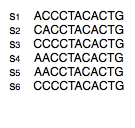
\includegraphics[width=100mm]{images/example1a}
  \end{center}
  \caption[An example showing two different {\sc Closest String} instances; one that is a motif set and one that is a decoy set.]{An example showing two different {\sc Closest String} instances; one that is a motif set (right) and one that is a decoy set (left).}
  \label{fig:motif_decoy_sets}
\end{figure}

Clearly, for a set $S$ to have at least one center string corresponding to the degeneracy parameter $d$, the Hamming distance between any pair of strings in $S$ must not exceed $2d$.  We refer to such a set of strings as being {\em pairwise bounded}. Determining whether a set of strings is pairwise bounded can be trivially decided in polynomial time and therefore, since the {\sc Closest String} problem is NP-complete, there must exist sets of strings that are pairwise bounded but do not contain a center string, unless P = NP.  In figure \ref{fig:motif_decoy_sets} there exist two sets of strings that are pairwise bounded when $d = 1$, however, the set on the left does not contain a length-$\ell$ string that has distance at most $d$ from each string in the set and the string on the right has such a string ({\em i.e.}\ the string in bold).  Thus, the {\sc Closest String} problem essentially reduces to discerning between pairwise bounded sets that have a center string (and if so, finding one such string) and those sets that do not. A set of strings $S$ is a {\em motif set} if there exists a center string and is a {\em decoy set} if $S$ is pairwise bounded but does not have a center string.

Also of considerable importance is the optimization version of the {\sc Closest String} problem.  Throughout this work, we will explicitly indicate when there exists ambiguity whether we are considering the optimization or decision version of the {\sc Closest String} problem. 

\begin{definition} {\bf (The Closest String Optimization Problem)} Given a set $S = \{s_1, s_2, \ldots, s_n\}$ of sequences, each of length $\ell$ and over an alphabet $\Sigma$, find a string $s$ of length $\ell$ over $\Sigma$ minimizing $d_c$ such that, for every string $s_i \in S$, $d(s, s_i) \leq d_c$. \end{definition}

We refer to the string $s$ in the context of the optimization version on the problem as the {\em center string}. 

\subsection{The {\sc Farthest String} Problem}

The {\sc Farthest String} problem was first introduced by Lanctot {\em et al.}\ \cite{LLMWZ00_v1}.  Whereas, the {\sc Closest String} problem abstractly defines the problem of finding a pattern that, with some error, occurs in one set of strings, the {\sc Farthest String} problem defines the problem where the pattern does not occur in a set of strings. Both of these string selection problems have application to the analysis of genomic data. The {\sc Farthest String} problem has been proved NP-complete even when the alphabet is binary  \cite{LLMWZ00_v1}, and therefore, it is unlikely to have an exact polynomial-time solution, unless P = NP. This problem can be more formally defined as follows: 

\begin{definition} {\bf (The Farthest String Problem) } Given a set $S_f$ of strings of length at least $\ell$ over an alphabet $\Sigma$ and a non-negative parameter $d_f$, the objective is to determine if there exists a string $s$ over the alphabet $\Sigma$  such that for any $s_i \in S_f$, $d(s, s_i) \geq d_f$.  \end{definition} 

Although the {\sc Farthest String} problem is not as well-studied as the {\sc Closest String} problem, it will be of both theoretical and practical interest in this thesis. 

\section{Biological Applications}

We introduced motif recognition by demonstrating its applicability to detecting transcription factor binding sites; however, there exist many other biological and non-biological applications for this problem. For example, motif recognition is applicable in the fields of coding theory \cite{CHLS97,FL97} and data compression \cite{GS85}.   There exist many other biological applications in addition to the ones discussed in this section, including finding an unbiased consensus of a protein family \cite{BLPR}, function prediction \cite{gusfield,asmith}, and modelling and predicting splice sites \cite{barnes}.

\subsubsection{Designing Diagnostic Probes}

Creating diagnostic probes for bacterial infection has been one of the core applications to the theoretical study of string selection and comparison problems \cite{BLPR,LLMWZ00,macario}.   Currently, oligonucleotide microarrays are being used in gene expression analysis, as well as for diagnostic purposes ({\em i.e.}\ the identification of micro-organisms in clinical and environmental samples). The key task is to efficiently determine suitable sets of oligonucleotide probes that can reliably detect and differentiate the target sequences.  Determining efficient algorithms that achieve this are of utmost importance since the datasets may be significantly large.  There exist algorithms to produce adequate probes when there exists a high amount of variability within the target sequences \cite{KS02,krause}; however, when the sequence database contains homologous genes, the problem still remains largely unsolved. In the case where it is impossible to determine specific probes due to the high similarity, it is advantageous to design probes that are specific for groups of closely related sequences, and that detect target sequences as well as some non-target sequences (referred to as negative probes).  Hence, given a set of DNA sequences from a group of closely related pathogenic bacteria and a host, the task is to find a sequence that occurs in each of the bacterial sequences without occurring in the host sequence.  

\subsubsection{Polymerase Chain Reaction}

Polymerase chain reaction (PCR) is a well-established technique in molecular biology to amplify a single or few copies of a DNA segment, referred to as a template, across several orders of magnitude, generating thousands to millions of copies of a particular DNA sequence. {\em Primers} are short DNA fragments that contain sequences complementary to the target region along with a DNA polymerase. Hence, they are key components which enable selective and repeated amplification. The DNA generated is itself used as a template for replication during the PCR by setting a chain reaction in which the DNA template is exponentially amplified. PCR can be modified to perform a wide array of genetic manipulations \cite{PH}. 

Creating universal PCR primers that are able to recognize multiple segments has been a problem well-investigated by the bioinformatics community \cite{DRSS,HMM,LLMWZ00,LBOT,PH}. The specificity of the primer hybridization directly affects the specificity of the amplification by PCR.  Designing well-constructed primers comes down to a sequence problem where one attempts to determine the maximum number of mismatches that can be allowed for hybridization.

\subsubsection{Drug Design}

Drug design is another biological application \cite{crooke,DLLM,LLMWZ00}.  Given a set of sequences of orthologous genes from a group of closely related pathogens, and a host, the goal is to find a subsequence that is highly conserved in all of the pathogen sequences but not conserved in the sequence of the host. This subsequence can in turn, be used to create a novel drug that harms several pathogens with minimal effect on the host.  


\section{Summary}

This thesis is focused on the development of combinatorial and probabilistic algorithms for problems arising from the analysis of genomic data. In particular, we will examine several traditional problems in bioinformatics, including motif recognition, {\sc Closest String}, and other string selection problems.  In this chapter we introduced each of these problems and motivated them by illustrating their application in biology.  Next, we will survey some of the important results through the literature pertinent to motif recognition, {\sc Closest String}, and its variants. 
